%\documentclass[handout]{beamer} %Makes Handouts
\usetheme{Singapore} %Gray with fade at top
\useoutertheme[subsection=false]{miniframes} %Supppress subsection in header
\useinnertheme{rectangles} %Itemize/Enumerate boxes
\usecolortheme{seagull} %Color theme
\usecolortheme{rose} %Inner color theme

\definecolor{light-gray}{gray}{0.75}
\definecolor{dark-gray}{gray}{0.55}
\setbeamercolor{item}{fg=light-gray}
\setbeamercolor{enumerate item}{fg=dark-gray}

\setbeamertemplate{navigation symbols}{}
\setbeamertemplate{mini frames}[default]
\setbeamercovered{dynamics}
\setbeamerfont*{title}{size=\Large,series=\bfseries}

%\setbeameroption{notes on second screen} %Dual-Screen Notes
%\setbeameroption{show only notes} %Notes Output

\newcommand{\heading}[1]{\noindent \textbf{#1}\\ \vspace{1em}}

\usepackage{bbding,color,multirow,times,ccaption,tabularx,graphicx,verbatim,booktabs,fixltx2e}
\usepackage{colortbl} %Table overlays
\usepackage[english]{babel}
\usepackage[latin1]{inputenc}
\usepackage[T1]{fontenc}

%\author[]{Thomas J. Leeper}
\institute[]{
  \inst{}%
  Department of Political Science and Government\\Aarhus University
}

\usepackage{tikz}
\usetikzlibrary{shapes,arrows}
\usetikzlibrary{decorations.pathreplacing}

\title{Methods Supplementary Lecture 2:\\Survey Analysis}

\date[]{}

\begin{document}

\frame{\titlepage}

\frame{\tableofcontents}

\section{Linear Regression Analysis}
\frame{\tableofcontents[currentsection]}


\frame{
	\frametitle{Uses of Regression}
	\begin{enumerate}\itemsep2em
	\item Description
	\item Prediction
	\item Causal Inference
	\end{enumerate}
}

\frame{
	\frametitle{Descriptive Inference}
	\begin{enumerate}\itemsep1em
	\item We want to understand a \textit{population} of cases
	\item We cannot observe them all, so:
		\begin{enumerate}
    		\item Draw a \textit{representative} sample
    		\item Perform mathematical procedures on sample data
    		\item Use assumptions to make inferences about population
    		\item Express uncertainty about those inferences based on assumptions
		\end{enumerate}
	\end{enumerate}
}

\frame{
	\frametitle{Parameter Estimation}
	\begin{itemize}\itemsep1em
    	\item We want to observe population \textit{parameter} $\theta$
    	\item If we obtain a representative sample of population units:\\
    		\begin{itemize}\itemsep1em
        		\item Our sample statistic $\hat{\theta}$ is an unbiased estimate of $\theta$
        		\item Our sampling procedure dictates how uncertain we are about the value of $\theta$
    		\end{itemize}
	\end{itemize}
}

\frame{
	\frametitle{An Example}
	\begin{itemize}
	\item We want to know $\bar{Y}$ (population mean)
	\item Our \textit{estimator} is the sample mean formula which produces the sample \textit{estimate} $\bar{y}$:
		\begin{equation}
		\bar{y} = \frac{1}{n}\sum_{i=1}^{n}y_i
		\end{equation}
	\item The \textit{sampling variance} is our uncertainty:
	\begin{equation}
	Var(\bar{y}) = \frac{s^2}{n}
	\end{equation}
	where $s^2 = $ sample element variance
	\end{itemize}
}

\frame{
	\frametitle{Uncertainty}
	\begin{itemize}\itemsep1em
		\item We never know $\theta$
		\item Our $\hat{\theta}$ is an estimate that may not equal $\theta$
			\begin{itemize}
    			\item Unbiased due to \textbf{Law of Large Numbers}
    			\item For $\bar{y}$: $N(Y, \sigma^2) $
			\end{itemize}
    	\item The size of sampling variance depends on:
    		\begin{itemize}
        		\item Element variance
        		\item Sample size!
    		\end{itemize}
    	\item Note: $SE(\bar{y}) = \sqrt{Var(\bar{y})}$
    	\item We may want to know $\hat{\theta}$ per se, but we are mostly interested in it as an estimate of $\theta$
	\end{itemize}
}

\frame{
	\frametitle{Causal Inference}
	\begin{enumerate}\itemsep1em
	\item<2-> Everything that goes into descriptive inference
	\item<3-> Plus, philosophical assumptions
	\item<4-> Plus, randomization \textit{or} perfectly specified model
	\end{enumerate}
}


\frame{\frametitle{Questions about philosophical assumptions?}}

\frame<1-5,2>[label=ways]{
	\frametitle{Ways of Thinking About OLS}
	\begin{enumerate}\itemsep1em
    	\item<2-> Estimating Unit-level Causal Effect
    	\item<3-> Ratio of $Cov(X,Y)$ and $Var(X)$
    	\item<4-> Minimizing residual sum of squares (SSR)
    	\item<5-> Line (or surface) of best fit
	\end{enumerate}
}


\frame{
	\frametitle{Bivariate Regression I}
	\begin{itemize}\itemsep1em
	\item $Y$ is continuous
	\item $X$ is a randomized treatment indicator/dummy $(0,1)$
	\item How do we know if the treatment $X$ had an effect on $Y$?
	\item<2-> Look at mean-difference: $E[Y_i|X_i=1] - E[Y_i|X_i=0]$
	\end{itemize}
}


\frame{
	\frametitle{Three Equations}
	\begin{enumerate}\itemsep2em
	\item Population: $Y = \beta_0 + \beta_1 X \hspace{0.5em} (+ \epsilon)$
	\item Sample estimate: $\hat{y} = \hat{\beta}_0 + \hat{\beta}_1 x$
	\item Unit:
		\begin{align*}
		y_i & = \hat{\beta}_0 + \hat{\beta}_1 x_i + e_i\\
		    & = \bar{y}_{0i} + (y_{1i} - y_{0i}) x_i + (y_{0i} - \bar{y}_{0i})
		\end{align*}
	\end{enumerate}
}


\frame<1-2>[label=dummy]{
	\frametitle{Bivariate Regression I}
	\begin{itemize}\itemsep1em
    	\item Mean difference ($E[Y_i|X_i=1] - E[Y_i|X_i=0]$) is the regression line slope
    	\item Slope ($\beta$) defined as $\frac{\Delta Y}{\Delta X}$
    		\vspace{1em}
    		\begin{itemize}\itemsep1em
        		\item<2-> $\Delta Y = E[Y_i|X=1] - E[Y_i|X=0]$
        		\item<2-> $\Delta X = 1 - 0 = 1$
    		\end{itemize}
    	\item<3-> How do we know if this is a \textit{significant} difference?
    		\begin{itemize}
        		\item We'll come back to that
    		\end{itemize}
	\end{itemize}

}

% graphs of mean-difference
% http://thomasleeper.com/regcourse/Slides-2014/Session02_01.html#20


\frame[label=bivariate1]{
	\begin{center}
	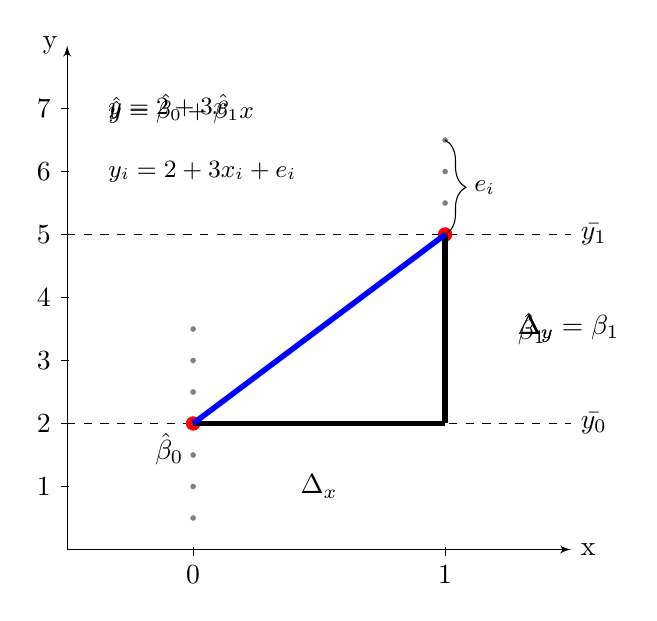
\begin{tikzpicture}[>=latex', scale=0.8]
        \draw[->] (0,0) node[below] (origin) {}  -- (8,0) node[right] (xaxis) {x};
        \draw[->] (origin) -- (0,8) node[left] (yaxis) {y};
        % x ticks
        \draw (2,1pt) -- (2,-3pt) node[anchor=north] {0};
        \draw (6,1pt) -- (6,-3pt) node[anchor=north] {1};
        % y ticks
        \foreach \y in {1,...,7}
             \draw (1pt,\y) -- (-3pt,\y) node[anchor=east] {$\y$};
        
        % points
        \foreach \y in {0.5,1.0,...,3.5} {
        	\draw[gray,fill] (2,\y) circle [radius=1pt];
        	\draw[gray,fill] (6,3+\y) circle [radius=1pt];
        }
        % y_0-bar
        \draw<2-4>[dashed] (0,2) -- (8,2) node[right] {$\bar{y_0}$};
        % y_1-bar
        \draw<2-4>[dashed] (0,5) -- (8,5) node[right] {$\bar{y_1}$};
        % mean points
        \draw<2->[red,fill] (2,2) circle [radius=3pt];
        \draw<2->[red,fill] (6,5) circle [radius=3pt];
        
        % slope
        \draw<3-4>[solid, line width=2pt] (2,2) -- (6,2);
        \draw<3-5>[solid, line width=2pt] (6,2) -- (6,5);
        \node<3-4>(deltax) at (4,1) {$\Delta_x$};
        \node<3>[right](deltay) at (7,3.5) {$\Delta_y$};
        \node<4>[right](deltay) at (7,3.5) {$\Delta_y = \beta_1$};
        \node<5>[right](deltay) at (7,3.5) {$\hat{\beta}_1$};
        
        \draw<4->[blue, solid, line width=2pt] (2,2) -- (6,5);
        \node<4-5>[below left](b0) at (2,2) {$\hat{\beta}_0$};
        
        \node<5>[right](eq) at (0.5,7) {\small $\hat{y} = \hat{\beta}_0 + \hat{\beta}_1 x$};
        \node<6->[right](eq) at (0.5,7) {\small $\hat{y} = 2 + 3 x$};
        \node<7->[right](eq) at (0.5,6) {\small $y_i = 2 + 3 x_i + e_i$};
        \draw<7->[right,decorate,decoration={brace,mirror,amplitude=7.5pt}] (6,5)  -- (6,6.5)
        	node [right, pos=0.5, xshift=7] {\small $e_i$};
    \end{tikzpicture}
    \end{center}
}

% OLS only makes sense in a linear world

\frame{
	\frametitle{Systematic versus unsystematic component of the data}
	\begin{itemize}\itemsep1em
    	\item Systematic: Regression line (slope)
    		\begin{itemize}
    		\item Linear regression estimates the conditional means of the population data (i.e., $E[Y|X]$)
    		\end{itemize}
    	\item Unsystematic: Error term is the deviation of observations from the line
    		\begin{itemize}
        		\item The difference between each value $y_i$ and $\hat{y}_i$ is the \textit{residual}: $e_i$
        		\item OLS produces an estimate of the relationship between X and Y that minimizes the \textit{residual sum of squares}
    		\end{itemize}
	\end{itemize}
}

\frame{
	\frametitle{Why are there residuals?}
	\begin{itemize}\itemsep1em
		\item<2-> Omitted variables
		\item<2-> Measurement error
		\item<2-> Fundamental randomness
	\end{itemize}
}

\againframe<2-3>{dummy}

\againframe<2-3>{ways}


\frame{
	\frametitle{Bivariate Regression II}
	\begin{itemize}\itemsep1em
	\item $Y$ is continuous
	\item $X$ is continuous (and randomized)
	\item How do we know if the treatment $X$ had an effect on $Y$?\\
		\begin{itemize}
		\item Correlation coefficient ($\rho$)
		\item Regression coefficient (slope; $\beta_1$)
		\end{itemize}
	\end{itemize}
}

\frame<1>[label=correlation]{
	\frametitle{Correlation Coefficient ($\rho$)}
	\begin{itemize}\itemsep1em
	\item Measures how well a scatterplot is represented by a straight (non-horizontal) line
	\item<2-> Formal definition: 
		$\frac{Cov(X,Y)}{\sigma_X \sigma_y}$
	\item<2-> As a reminder:\\
		\begin{itemize}\itemsep1em
		\item $Cov(x,y) = \sum_{i=1}^{n}(x_i - \bar{x})(y_i - \bar{y})$
		\item $s_x = \sqrt{\sum_{i=1}^{n}(x_i - \bar{x})^2}$
		\end{itemize}
	\end{itemize}
}

\frame{
	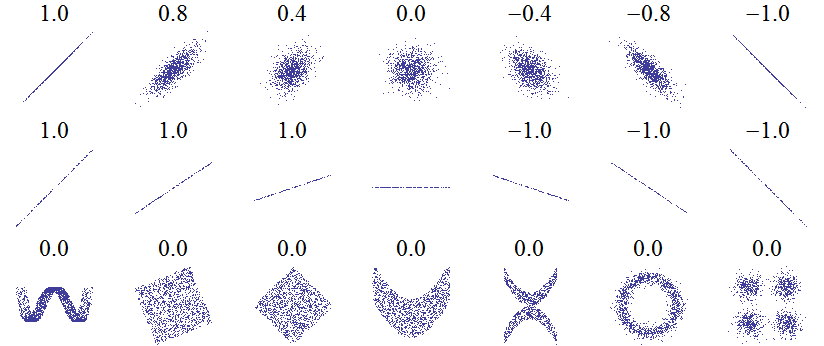
\includegraphics[width=\textwidth]{images/correlation}
}

\againframe<1->{correlation}

\frame{
	\frametitle{OLS Coefficient ($\beta_1$)\footnote{Multivariate formula involves matrices; Week 20}}
	\begin{itemize}\itemsep1em
	\item Measures $\Delta Y$ given $\Delta X$
	\item<2-> Formal definition: 
		$\frac{Cov(X,Y)}{Var(X)}$
	\item<2-> As a reminder:\\
		\begin{itemize}\itemsep1em
		\item $Cov(x,y) = \sum_{i=1}^{n}(x_i - \bar{x})(y_i - \bar{y})$
		\item $Var(x) = \sum_{i=1}^{n}(x_i - \bar{x})^2$
		\end{itemize}
	\item<3-> $\hat{\rho}$ and $\hat{\beta_1}$ are just scaled versions of $\widehat{Cov}(x,y)$
	\end{itemize}
}

\frame<1-6>[label=math]{
	\frametitle{Minimum Mathematical Requirements}
	\begin{enumerate}\itemsep1em
    	\item<1-> Do we need variation in $X$?
    		\begin{itemize}
        		\item<2-> Yes, otherwise dividing by zero
    		\end{itemize}
    	\item<3-> Do we need variation in $Y$?
    		\begin{itemize}
        		\item No, $\hat{\beta}_1$ can equal zero
    		\end{itemize}
    	\item<5-> How many observations do we need?
    		\begin{itemize}
    		\item<6-> $n \ge k$, where $k$ is number of parameters to be estimated
    		\end{itemize}
    	\item<7-> Can we have highly correlated regressors?
    		\begin{itemize}
    		\item<8-> Generally no (due to multicollinearity)
    		\end{itemize}
	\end{enumerate}
}

\frame<1-5>[label=scatter]{
	\begin{center}
	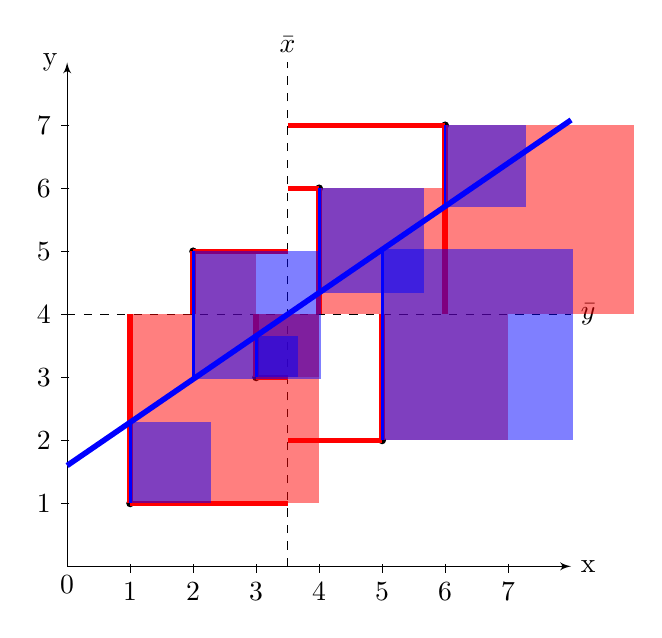
\begin{tikzpicture}[>=latex', scale=0.8]
        \draw[->] (0,0) node[below] (origin) {0}  -- (8,0) node[right] (xaxis) {x};
        \draw[->] (origin) -- (0,8) node[left] (yaxis) {y};
        % x ticks
        \foreach \x in {1,...,7}
        	\draw (\x,1pt) -- (\x,-3pt) node[anchor=north] {$\x$};
        % y ticks
        \foreach \y in {1,...,7}
             \draw (1pt,\y) -- (-3pt,\y) node[anchor=east] {$\y$};
        % points
        \draw[fill] (1,1) circle [radius=1.5pt];
        \draw[fill] (2,5) circle [radius=1.5pt];
        \draw[fill] (3,3) circle [radius=1.5pt];
        \draw[fill] (4,6) circle [radius=1.5pt];
        \draw[fill] (5,2) circle [radius=1.5pt];
        \draw[fill] (6,7) circle [radius=1.5pt];
        % x-bar
        \draw<2->[dashed] (3.5, 0) -- (3.5,8) node[above] {$\bar{x}$};
        % y-bar
        \draw<2->[dashed] (0,4) -- (8,4) node[right] {$\bar{y}$};
        
        % x-deviations
        \draw<3>[red, line width=2pt] (1,1) -- (3.5,1);
        \draw<3>[red, line width=2pt] (2,5) -- (3.5,5);
        \draw<3>[red, line width=2pt] (3,3) -- (3.5,3);
        \draw<3>[red, line width=2pt] (4,6) -- (3.5,6);
        \draw<3>[red, line width=2pt] (5,2) -- (3.5,2);
        \draw<3>[red, line width=2pt] (6,7) -- (3.5,7);
        % y-deviations
        \draw<4,6-7,10-11>[red, line width=2pt] (1,1) -- (1,4);
        \draw<4,6-7,10-11>[red, line width=2pt] (2,5) -- (2,4);
        \draw<4,6-7,10-11>[red, line width=2pt] (3,3) -- (3,4);
        \draw<4,6-7,10-11>[red, line width=2pt] (4,6) -- (4,4);
        \draw<4,6-7,10-11>[red, line width=2pt] (5,2) -- (5,4);
        \draw<4,6-7,10-11>[red, line width=2pt] (6,7) -- (6,4);
        
		\fill<7,11>[red, opacity=0.5] (1,1) rectangle (4,4);
		\fill<7,11>[red, opacity=0.5] (2,5) rectangle (3,4);
		\fill<7,11>[red, opacity=0.5] (3,3) rectangle (4,4);
		\fill<7,11>[red, opacity=0.5] (4,6) rectangle (6,4);
		\fill<7,11>[red, opacity=0.5] (5,2) rectangle (7,4);
		\fill<7,11>[red, opacity=0.5] (6,7) rectangle (9,4);

        % line
        \draw<5->[blue, line width=2pt] (0,1.6) -- (8,7.0856);
        
        % residuals
        \draw<8->[blue, line width=1pt] (1,1) -- (1,2.29);
        \draw<8->[blue, line width=1pt] (2,5) -- (2,2.97);
        \draw<8->[blue, line width=1pt] (3,3) -- (3,3.66);
        \draw<8->[blue, line width=1pt] (4,6) -- (4,4.34);
        \draw<8->[blue, line width=1pt] (5,2) -- (5,5.03);
        \draw<8->[blue, line width=1pt] (6,7) -- (6,5.71);
		
		\fill<9-11>[blue, opacity=0.5] (1,1) rectangle (2.29,2.29);
		\fill<9-11>[blue, opacity=0.5] (2,5) rectangle (4.03,2.97);
		\fill<9-11>[blue, opacity=0.5] (3,3) rectangle (3.66,3.66);
		\fill<9-11>[blue, opacity=0.5] (4,6) rectangle (5.66,4.34);
		\fill<9-11>[blue, opacity=0.5] (5,2) rectangle (8.03,5.03);
		\fill<9-11>[blue, opacity=0.5] (6,7) rectangle (7.29,5.71);

		
    \end{tikzpicture}
    \end{center}
}

\frame{
	\frametitle{Calculations}
	\begin{tabular}{rrrrrr} \hline
	$x_i$ & $y_i$ & $x_i - \bar{x}$ & $y_i - \bar{y}$ & $(x_i - \bar{x})(y_i - \bar{y})$ & $(x_i - \bar{x})^2$\\ \hline
	1 & 1 & ? & ? & ? & ? \\
	2 & 5 & ? & ? & ? & ? \\
	3 & 3 & ? & ? & ? & ? \\
	4 & 6 & ? & ? & ? & ? \\
	5 & 2 & ? & ? & ? & ? \\
	6 & 7 & ? & ? & ? & ? \\ \hline
	\end{tabular}
}
% mean(x) = 3.5
% mean(y) = 4
% cov(x,y) = 12
% var(x) = 17.5
% slope = 0.6857143

\frame{
	\frametitle{Intercept $\hat{\beta}_0$}
	\begin{itemize}\itemsep1em
	\item Simple formula: $\hat{\beta}_0 = \bar{y} - \hat{\beta}_1 \bar{x}$
	\item<2-> Intuition: OLS fit always runs through point $(\bar{x}, \bar{y})$
	\item<3-> Ex.: $\hat{\beta}_0 = 4 - 0.6857 * 3.5 = 1.6$
	\item<4-> $\hat{y} = 1.6 + 0.6857 \hat{x}$
	\end{itemize}
}

\againframe<5>{scatter}

% CEF: compare $\bar{Y}$ and $E[Y|X=x]$

\againframe<3-4>{ways}


\frame{
	\frametitle{OLS Minimizes SSR}
	\begin{itemize}\itemsep1em
    	\item Total Sum of Squares (SST): $\sum_{i=1}^{n}(y_i - \bar{y})^2$
    	\item We can partition SST into two parts (ANOVA):
    		\begin{itemize}
    		\item Explained Sum of Squares (SSE)
    		\item Residual Sum of Squares (SSR)
    		\end{itemize}
    	\item $SST = SSE + SSR$
    	\item OLS is the line with the lowest SSR
	\end{itemize}
}

\againframe<5-11>{scatter}

\frame{\frametitle{Questions about OLS calculations?}}


\frame[label=anygood]{
	\frametitle{Are Our Estimates Any Good?}
	Yes, if:\\
	\begin{enumerate}\itemsep1em
   		\item Works mathematically
   		\item Causally valid theory
   		\item Linear relationship between $X$ and $Y$
   		\item $X$ is measured without error
   		\item No missing data (or MCAR; see Lecture 5)
   		\item No confounding
	\end{enumerate}
}


\frame{
	\frametitle{Linear Relationship}
	\begin{itemize}\itemsep1em
    	\item If linear, no problems
    	\item If non-linear, we need to transform
    		\begin{itemize}
        		\item Power terms (e.g., $x^2$, $x^3$)
        		\item log (e.g., $log(x)$)
        		\item Other transformations
        		\item If categorical: convert to set of indicators
        		\item Multivariate interactions (next week)
    		\end{itemize}
	\end{itemize}
}

\frame{
	\frametitle{Coefficient Interpretation Activity}
	\begin{itemize}\itemsep1em
	\item Four types of variables:
		\begin{enumerate}
		\item Indicator (0,1)
		\item Categorical
		\item Ordinal
		\item Interval
		\end{enumerate}
	\item How do we interpret a coefficient on each of these types of variables?
	\end{itemize}
}

\frame{
	\frametitle{Notes on Interpretation}
	\begin{itemize}\itemsep1em
	\item<1-> Effect $\beta_1$ is constant across values of $x$
	\item<2-> That is not true when there are:
		\begin{itemize}
		\item Interaction terms (next week)
		\item Nonlinear transformations (e.g., $x^2$)
		\item Nonlinear regression models (e.g., logit/probit)
		\end{itemize}
	\item<3-> Interpretations are sample-level
		\begin{itemize}
		\item Sample representativeness determines generalizability
		\end{itemize}
	\item<4-> Remember uncertainty
		\begin{itemize}
		\item These are \textit{estimates}, not population parameters
		\end{itemize}
	\end{itemize}
}



\frame{
	\frametitle{Measurement Error in Regressor(s)}
	\begin{itemize}\itemsep1em
    	\item We want effect of $x$, but we observe $x^{*}$, where $x = x^{*} + w$:
    	\begin{align*}
    	y & = \beta_0 + \beta_1 x^{*} + \epsilon\\
    	 & = \beta_0 + \beta_1 (x - w) + \epsilon\\
    	 & = \beta_0 + \beta_1 x + (\epsilon - \beta_1 w)\\
    	 & = \beta_0 + \beta_1 x + v
    	\end{align*}
	\end{itemize}
}

\frame{
	\frametitle{Measurement Error in Regressor(s)}
	\begin{itemize}\itemsep1em
    	\item Produces \textit{attenuation}: as measurement error increases, $\beta_1 \rightarrow 0$
    	\item Our coefficients fit the observed data
    	\item But they are \textit{biased} estimates of our population equation
    		\begin{itemize}
    		\item This applies to all $\hat{\beta}$ in a multivariate regression
    		\item Direction of bias is unknown
    		\end{itemize}
	\end{itemize}
}


\frame{
	\frametitle{Measurement Error in $Y$}
	\begin{itemize}\itemsep1em
    	\item Not necessarily a problem
    	\item If \textit{random} (i.e., uncorrelated with $x$), it costs us precision
    	\item If \textit{systematic}, who knows?!
    	\item If \textit{censored}, see Lectures 11 and/or 12
	\end{itemize}
}


\frame{
	\frametitle{Missing Data}
	\begin{itemize}\itemsep1em
	\item Missing data can be a big problem
	\item We will discuss it in Lecture 5
	\end{itemize}
}

\frame{
	\frametitle{Confounding (Selection Bias)}
	\begin{itemize}\itemsep1em
	\item If $x$ is not randomly assigned, potential outcomes are not independent of $x$
	\item Other factors explain why a unit $i$ received their particular value $x_i$
	\vspace{1em}
	\item In matching, we obtain this \textit{conditional independence} by comparing units that are identical on all confounding variables
	\end{itemize}
}

\frame{
	\frametitle{Omitted Variables}
	{\small
	$\underbrace{E[Y_i| X_i = 1] - E[Y_i | X_i = 0] =}_{\text{Naive Effect}}$\\
	\vspace{1em}
	$\underbrace{E[Y_{1i}|X_i =1] - E[Y_{0i} | X_i = 1]}_{\text{Treatment Effect on Treated (ATT)}} + \underbrace{E[Y_{0i}|X_i = 1] - E[Y_{0i}|X_i=0]}_{\text{Selection Bias}}$
	}
	\vspace{1em}
}

\frame[label=causalgraph]{
	\begin{center}
	\begin{tikzpicture}[>=latex',circ/.style={draw, shape=circle, node distance=5cm, line width=1.5pt}]
        \draw[->] (0,0) node[left] (X) {X} -- (2.5,0) node[right] (D) {D};
        \draw[->] (3.1,0) -- (5,0) node[right] (Y) {Y};
        \draw[->] (-3,4) node[above] (Z) {Z} -- (X);
        \draw[->] (Z) -- (Y);
        \draw[->] (5,2) node[above] (A) {A} -- (Y);
        \draw[->] (-2,0) node[left] (B) {B} -- (X);
        \draw[->] (X) -- (2,-2) node[right] (C) {C};
    \end{tikzpicture}
    \end{center}
}

\frame{
	\frametitle{Omitted Variable Bias}
	\begin{itemize}
	\item We want to estimate:
	\begin{align*}
	Y = \beta_0 + \beta_1 X + \beta_2 Z + \epsilon
	\end{align*}
	\item We actually estimate:
	\begin{align*}
	\tilde{y} & = \tilde{\beta_0} + \tilde{\beta_1} x + \epsilon\\
	& = \tilde{\beta_0} + \tilde{\beta_1} x + (0 * z) + \epsilon\\
	& = \tilde{\beta_0} + \tilde{\beta_1} x + \nu
	\end{align*}
	\item Bias: $\tilde{\beta}_1 = \hat{\beta}_1 + \hat{\beta}_2 \tilde{\delta}_1$, where $\tilde{z} = \tilde{\delta}_0 + \tilde{\delta}_1 x$
	\end{itemize}
}

\frame{
	\frametitle{Size and Direction of Bias}
	\begin{itemize}
	\item Bias: $\tilde{\beta}_1 = \hat{\beta}_1 + \hat{\beta}_2 \tilde{\delta}_1$, where $\tilde{z} = \tilde{\delta}_0 + \tilde{\delta}_1 x$
	\end{itemize}
	\vspace{1em}
	\begin{center}
	\begin{tabular}{lll}
		              & $Corr(x,z)<0$ & $Corr(x,z)>0$ \\ \hline
		$\beta_2 < 0$ & Positive      & Negative      \\
		$\beta_2 > 0$ & Negative      & Positive      \\ \hline
	\end{tabular}
	\end{center}
}


\frame{
	\frametitle{Aside: Three Meanings of ``Endogeneity''}
	Formally endogeneity is when $Cov(X,\epsilon) \neq 0$
	\vspace{1em}
	\begin{enumerate}\itemsep1em
	\item Measurement error in regressors
	\item Omitted variables associated with included regressors 
		\begin{itemize}
		\item ``Specification error''
		\item Confounding
		\end{itemize}
	\item Lack of temporal precedence
	\end{enumerate}
}




\frame{
	\frametitle{Common Conditioning Strategies}
	\begin{enumerate}\itemsep1em
    	\item<2-> Condition on nothing (``naive effect'')
    	\item<3-> Condition on some variables
    	\item<4-> Condition on all observables
	\end{enumerate}
	\vspace{1em}
	\onslide<5->{Which of these are good strategies?}
}


\frame<1-2>[label=what]{
	\frametitle{What goes in our regression?}
	\begin{itemize}\itemsep1em
    	\item Use theory to build causal models
    		\begin{itemize}
    		\item Often, a causal graph helps
    		\end{itemize}
    	\item Some guidance:
    		\begin{itemize}
    		\item<2-> Include confounding variables
	    	\item<3-> Do not include post-treatment variables
	    	\item<4-> Do not include \textit{colinear} variables
    		\item<5-> Including irrelevant variables costs certainty
    		\item<6-> Including variables that affect $Y$ alone increases certainty
    		\end{itemize}
	\end{itemize}
}

\againframe{causalgraph}

\againframe<2-3>{what}

\againframe{causalgraph}

\frame{
	\frametitle{Post-treatment Bias}
	\begin{itemize}\itemsep1em
	\item We usually want to know the \textbf{total effect} of a cause
	\item If we include a mediator, $D$, of the $X \rightarrow Y$ relationship, the coefficient on $X$:
		\begin{itemize}
    		\item Only reflects the \textbf{direct} effect
    		\item Excludes the \textbf{indirect} effect of $X$ through $M$
		\end{itemize}
	\item So don't control for mediators!
	\end{itemize}
}

\againframe<3-4>{what}

\againframe<6-8>{math}

\againframe<4-6>{what}

\againframe{causalgraph}

\frame{
	\frametitle{Multivariate Regression Interpretation}
	\begin{itemize}\itemsep1em
	\item All our interpretation rules from earlier still apply in a multivariate regression
	\item Now we interpret a coefficient as an effect ``all else constant''
	\item Generally, not good to give all coefficients a causal interpretation
		\begin{itemize}
		\item Think ``forward causal inference''
		\item We're interested in the $X \rightarrow Y$ effect
		\item All other coefficients are there as ``controls''
		\end{itemize}
	\end{itemize}
}

\frame{
	\frametitle{From Line to Surface I}
	\begin{itemize}\itemsep1em
	\item In simple regression, we estimate a \textbf{line}
	\item In multiple regression, we estimate a \textbf{surface}
	\item Each coefficient is the \textit{marginal effect}, all else constant (at mean)
	\item This can be hard to picture in your mind
	\end{itemize}
}

\frame{
	\frametitle{From Line to Surface II}
	\begin{center}
	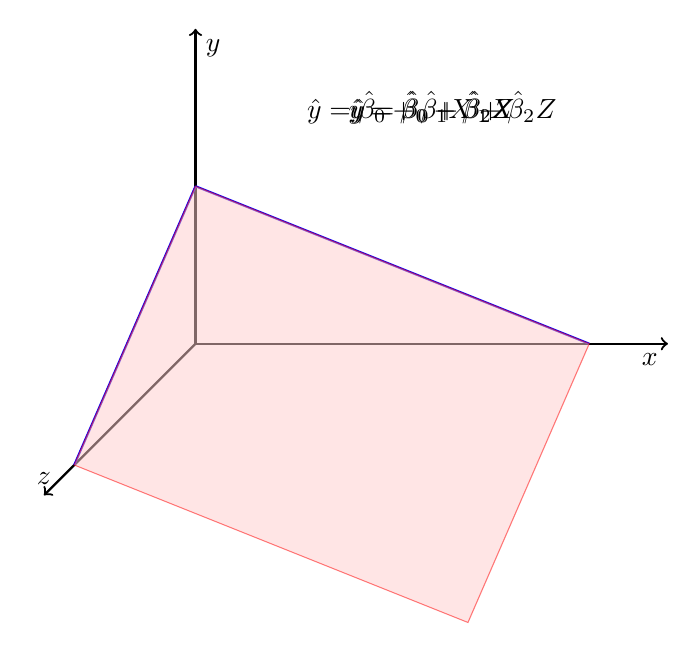
\begin{tikzpicture}
	    \draw[thick,->] (0,0,0) -- (6,0,0) node[anchor=north east]{$x$};
	    \draw[thick,->] (0,0,0) -- (0,4,0) node[anchor=north west]{$y$};
	    \draw<1> (3,3,0) node {$\hat{y} = \hat{\beta}_0 + \hat{\beta}_1 X$};
        \draw<2> (3,3,0) node {$\hat{y} = \hat{\beta}_0 + \hat{\beta}_2 Z$};
	    \draw<3> (3,3,0) node {$\hat{y} = \hat{\beta}_0 + \hat{\beta}_1 X + \hat{\beta}_2 Z$};
	    \draw<1,3>[thick, blue] (0,2,0) -- (5,0,0);
	    \draw<2->[thick,->] (0,0,0) -- (0,0,5) node[anchor=south]{$z$};
	    \draw<2->[thick, blue] (0,2,0) -- (0,0,4);
	    \filldraw<3->[draw=red,fill=red!20,opacity=0.5]
	        (0,2,0) -- (0,0,4) -- (5,-2,4) -- (5,0,0) -- cycle;
	\end{tikzpicture}
	\end{center}
}


\againframe{anygood}

\frame{
	\frametitle{OLS is BLUE}
	\begin{itemize}\itemsep1em
	\item BLUE: Best Linear Unbiased Estimator
	\item Gauss Markov Assumptions:
		\begin{enumerate}
		\item Linearity in parameters
		\item Random sampling
		\item No multicollinearity
		\item Exogeneity ($E[\epsilon|\mathbf{X}] = 0$)
		\item Homoskedasticity ($Var(\epsilon|\mathbf{X}) = \sigma^2$)
		\end{enumerate}
	\item Assumptions 1--4 prove OLS is unbiased
	\item Assumption 5 proves OLS is the \textit{best} estimator
	\end{itemize}
}



\frame{
	\frametitle{Squared vs. Absolute Errors}
	\begin{itemize}\itemsep1em
	\item Conventionally use Sum of Squared Errors
	\item Using absolute errors is also unbiased
	\item Sum of Squared Errors:
		\begin{itemize}
		\item more heavily weights outliers
		\item has a smaller variance
		\end{itemize} 
	\item Thus OLS is \textbf{B}est\textbf{LUE}
	\end{itemize}
}







\section{Goodness-of-Fit}
\frame{\tableofcontents[currentsection]}

\frame{
	\frametitle{Goodness-of-Fit}
	\begin{itemize}\itemsep1em
	\item We want to know: ``How good is our model?''
	\item<2-> We can answer:\\
		``How well does our model fit the observed data?''
	\item<3-> Is this what we want to know?
	\end{itemize}
}

\frame{
	\frametitle{Correlation}
	\begin{itemize}\itemsep1em
	\item Definition: $Corr(x,y) = \hat{r}_{x,y} = \frac{Cov(x,y)}{(n-1) s_x s_y}$
	\item Slope $\hat{\beta}_1$ and correlation $\hat{r}_{x,y}$ are simply different scalings of $Cov(x,y)$
	\item Interpretation: How well the bivariate relationship is summarized by a cloud of points?
	\item Units: none (range -1 to 1)
	\end{itemize}
}

\frame{
	\frametitle{Coefficient of Determination ($R^2$)}
	\begin{itemize}\itemsep1em
	\item Definition: $R^2 = \hat{r}_{x,y}^2 = \frac{SSE}{SST} = 1 - \frac{SSR}{SST}$
	\item Interpretation: How much of the total variation in $y$ is explained by the model?
	\item But, $R^2$ increases simply by adding more variables
	\item So, Adjusted-$R^2 = R^2 - (1 - R^2)\frac{k}{n-k-1}$, where $k$ is number of regressors
	\item Units: none (range 0 to 1)
	\end{itemize}
}

\frame{
	\frametitle{Standard Error of the Regression (SER)}
	\begin{itemize}\itemsep1em
	\item ``Root mean squared error'' or just $\sigma$
	\item Definition: $\hat{\sigma} = \sqrt{\frac{SSR}{n-p}}$, where $p$ is number of parameters estimated
	\item Interpretation: How far, on average, are the observed $y$ values from their corresponding fitted values $\hat{y}$
		\begin{itemize}
		\item $sd(y)$ is how far, on average, a given $y_i$ is from $\bar{y}$
		\item $\sigma$ is how far, on average, a given $y_i$ is from $\hat{y}_i$
		\end{itemize}
	\item Units: same as $y$ (range 0 to $sd(y)$)
	\end{itemize}
}

\frame{
	\frametitle{The F-test}
	\begin{itemize}\itemsep1em
	\item Definition: Test of whether any of our coefficients differ from zero
		\begin{itemize}
		\item In a bivariate regression, $F=t^2$
		\end{itemize}
	\item Interpretation: Do any of the coefficients differ from zero?
		\begin{itemize}
		\item Not a very interesting measure
		\end{itemize}
	\item Units: none (range 0 to $\infty$)
	\end{itemize}
}



\section{Generalized Linear Models}
\frame{\tableofcontents[currentsection]}

\frame{\frametitle{}}
\frame{
    \frametitle{Non-continuous Outcomes}
    \begin{enumerate}\itemsep1em
    \item Why shouldn't we use OLS for a non-continuous outcome variable?
    \item<2-> What do we do instead?
        \begin{itemize}
        \item<3-> Use a generalized linear model (GLM)
        \end{itemize}
    \end{enumerate}
}


\frame{
    \frametitle{Regression on a Latent Variable}
    \begin{itemize}\itemsep1em
    \item Consider a binary outcome $y$ (e.g., voting)
    \item OLS provides a nonsensical fit to the outcome
    \item Think about the problem as a ``latent'' outcome ($y\ast$) that manifests in two observed categories
        \begin{itemize}
        \item As $y\ast$ increases, $Pr(Y=1) \rightarrow 1$
        \item As $y\ast$ decreases, $Pr(Y=1) \rightarrow 0$
        \end{itemize}
    \item We do not observe $y\ast$, only $y$
    \end{itemize}
}

\frame{
    \frametitle{Estimation in GLM}
    \begin{itemize}\itemsep1em
    \item In OLS, we estimate: $\hat{y} = \beta_0 + \beta_1 x + e$
    \item This represents the conditional mean of $y$
    \item In a GLM, we estimate: $\hat{y}\ast = \beta_0 + \beta_1 x + e$\\
    where $y\ast$ is a transformation of $y$
    \item This is also a prediction of the conditional mean of $y$
    \item<2-> How do we transform $y$ to $y\ast$?
    \end{itemize}
}

\frame{
    \frametitle{Model Specification}
    \begin{enumerate}\itemsep1em
    \item<1-> Complete set of conditioning variables
    \item<2-> Correctly specified model
    \item<3-> Choice of error distribution
    \item<4-> Link function
    \end{enumerate}
}

\frame{
	\frametitle{Error Distribution}
	\begin{itemize}\itemsep1em
	\item To estimate a linear model using OLS, no distributional assumption is needed
	\item We can use Maximum Likelihood Estimation to obtain identical coefficient estimates as OLS by assuming errors are Normally distributed
    	\begin{itemize}
    	\item $\dfrac{1}{\sigma\sqrt{2\pi}} e^{-\dfrac{(x-\mu)^2}{2\sigma^2}}$
    	\end{itemize}
	\item For any GLM, we must assume the population distribution of the errors
    	\begin{itemize}
    	\item In almost all cases, an \textit{exponential family} distribution
    	\item i.e., a bell-shaped distribution that is not Normal
    	\end{itemize}
	\end{itemize}
}


\frame{
    \frametitle{Link Function}
    \begin{itemize}\itemsep2em
    \item $y\ast = X\beta = \beta_0 + \beta_1 x_1 + \beta_2 x_2 + \dots$
    \item \textbf{Link function}: $g(\mu) = X\beta$
        \begin{itemize}
        \item Transforms $y$ to $y\ast$
        \end{itemize}
    \item \textbf{Inverse link function}: $\mu = g^{-1}(X\beta)$
        \begin{itemize}
        \item Transforms $y\ast$ back to $y$
        \end{itemize}
    \end{itemize}
}


\begin{frame}[fragile]
    \frametitle{Inverse Link Function}
    
    \begin{itemize}
    \item This plot displays $g^{-1}(0.75x)$, where $g^{-1}$ is the inverse logit link.
    \end{itemize}
    
    \begin{center}
    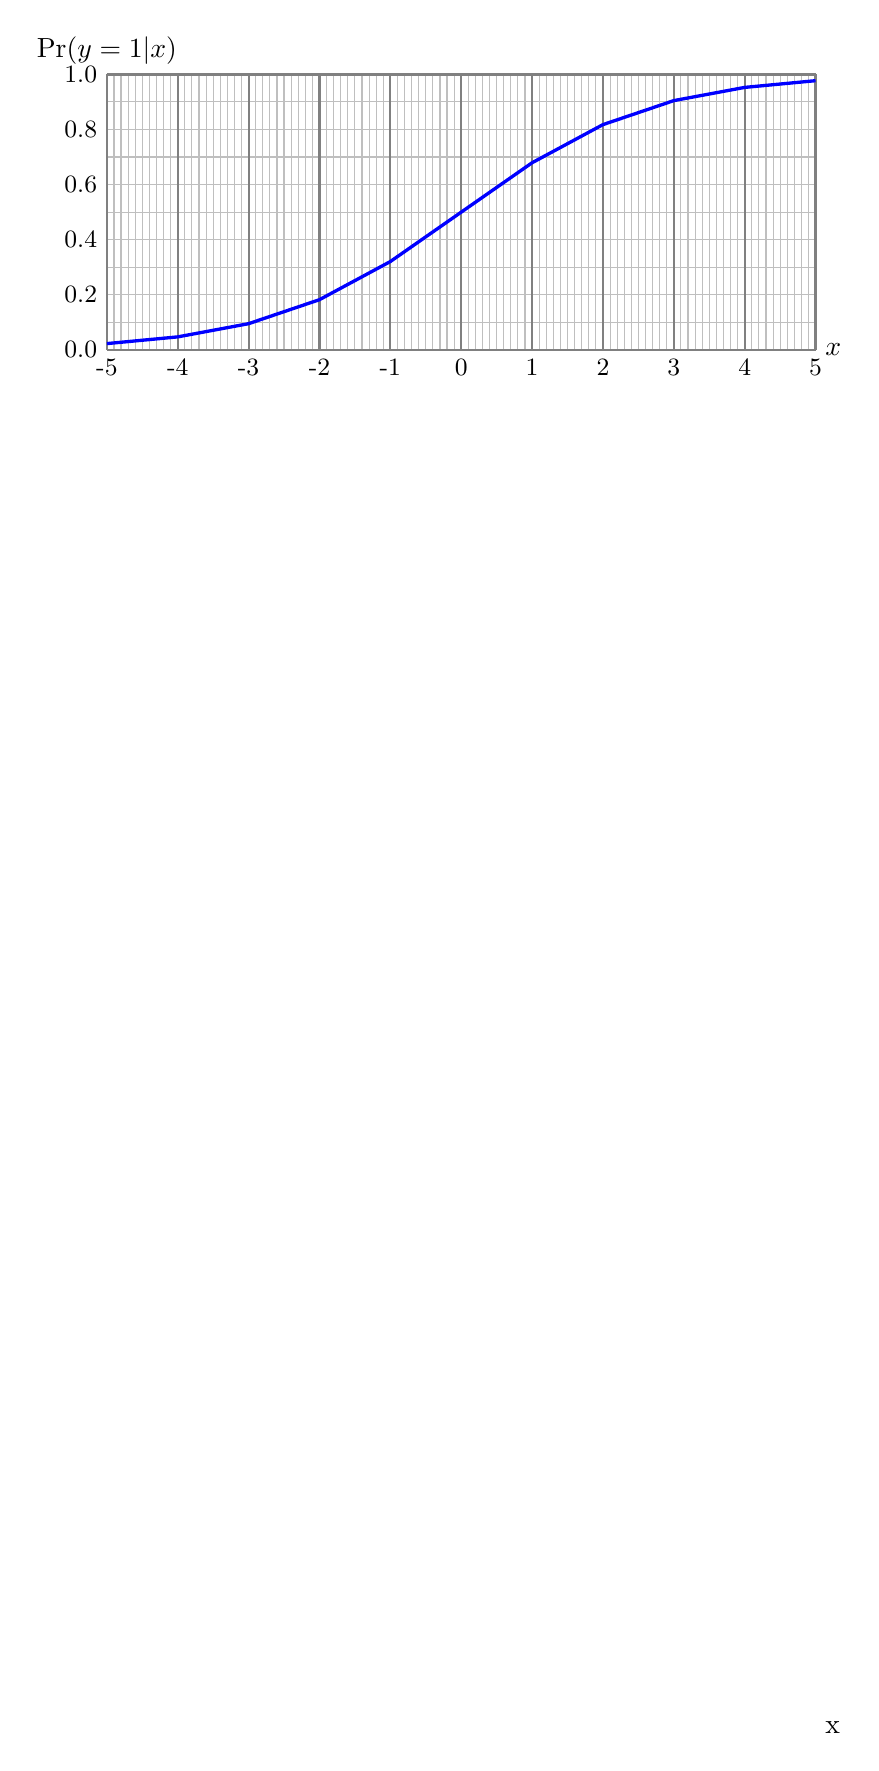
\begin{tikzpicture}[yscale=3.5, xscale=0.9]
    \draw [thin, step=0.1, lightgray] (-5,0) grid (5,1);
    \draw [thick, gray] (-5,0) grid (5,1);
    \node[right] () at (5,-5) {x};
    \node[right] () at (5,0) {$x$};
    \node[above] () at (-5,1) {$\Pr(y=1|x)$};
    \foreach \x in {-5,...,5} {
        \node[below] () at (\x,0) {\small \x};
    }
    \foreach \y in {0.0,0.2,0.4,0.6,0.8,1.0} {
    \node[left] () at (-5,\y) {\small \y};
    }
    % paste0("(", -5:5, ",", round(plogis(0.75*(-5:5)),4), ")", collapse = " -- ")
    \draw [very thick, blue] (-5,0.023) -- (-4,0.0474) -- (-3,0.0953) -- (-2,0.1824) -- (-1,0.3208) -- (0,0.5) -- (1,0.6792) -- (2,0.8176) -- (3,0.9047) -- (4,0.9526) -- (5,0.977);
    \end{tikzpicture}
    \end{center}
\end{frame}

\begin{frame}[fragile]
    \frametitle{From $x$ to Linear Prediction ($y\ast$)}
    \begin{center}
    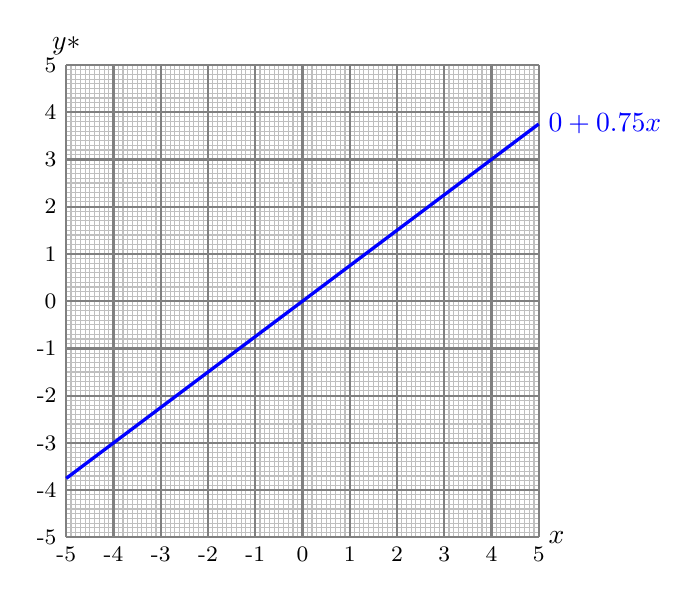
\begin{tikzpicture}[scale=0.6]
    \draw [thin, step=0.1, lightgray] (-5,-5) grid (5,5);
    \draw [thick, gray] (-5,-5) grid (5,5);
    \node[right] () at (5,-5) {$x$};
    \node[above] () at (-5,5) {$y\ast$};
    \foreach \x in {-5,...,5} {
        \node[below] () at (\x,-5) {\footnotesize \x};
    }
    \foreach \y in {-5,...,5} {
    \node[left] () at (-5,\y) {\footnotesize \y};
    }
    % paste0("(", -5:5, ",", round(0.75*(-5:5),4), ")", collapse = " -- ")
    \draw [very thick, blue] (-5,-3.75) -- (-4,-3) -- (-3,-2.25) -- (-2,-1.5) -- (-1,-0.75) -- (0,0) -- (1,0.75) -- (2,1.5) -- (3,2.25) -- (4,3) -- (5,3.75);
    \node[right,blue] () at (5,3.75) {$0 + 0.75x$};
    \end{tikzpicture}
    \end{center}
\end{frame}


\begin{frame}[fragile]
    \frametitle{From $y\ast$ to $Pr(y=1)$}
    \begin{center}
    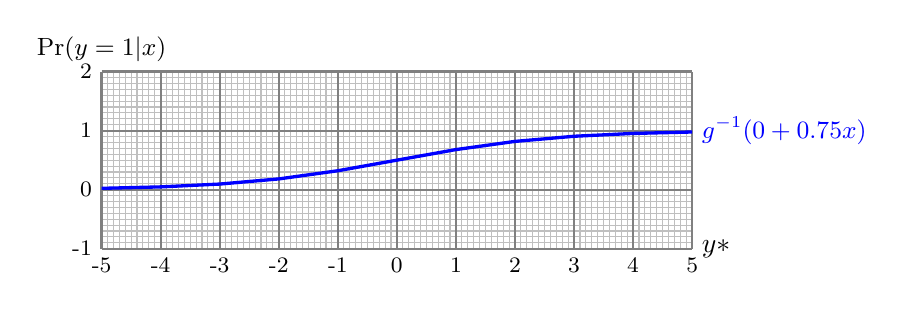
\begin{tikzpicture}[scale=0.75]
    \draw [thin, step=0.1, lightgray] (-5,-1) grid (5,2);
    \draw [thick, gray] (-5,-1) grid (5,2);
    \node[right] () at (5,-1) {$y\ast$};
    \node[above] () at (-5,2) {\small $\Pr(y=1|x)$};
    \foreach \x in {-5,...,5} {
        \node[below] () at (\x,-1) {\footnotesize \x};
    }
    \foreach \y in {-1,...,2} {
    \node[left] () at (-5,\y) {\footnotesize \y};
    }
    % paste0("(", -5:5, ",", round(plogis(0.75*(-5:5)),4), ")", collapse = " -- ")
    \draw [very thick, blue] (-5,0.023) -- (-4,0.0474) -- (-3,0.0953) -- (-2,0.1824) -- (-1,0.3208) -- (0,0.5) -- (1,0.6792) -- (2,0.8176) -- (3,0.9047) -- (4,0.9526) -- (5,0.977);
    \node[right,blue] () at (5,1) {\small $g^{-1}(0 + 0.75x)$};
    \end{tikzpicture}
    \end{center}
    
    \begin{itemize}
    \item Function is monotonic
    \item There is a \textit{cutpoint} in $y\ast$ where $\Pr(y) = 0.5$
    \item It is symmetric above and below the cutpoint
    \end{itemize}
\end{frame}


\begin{frame}[fragile]
    \frametitle{Putting it Together}
    \vspace{-1.5em}
    \begin{center}
    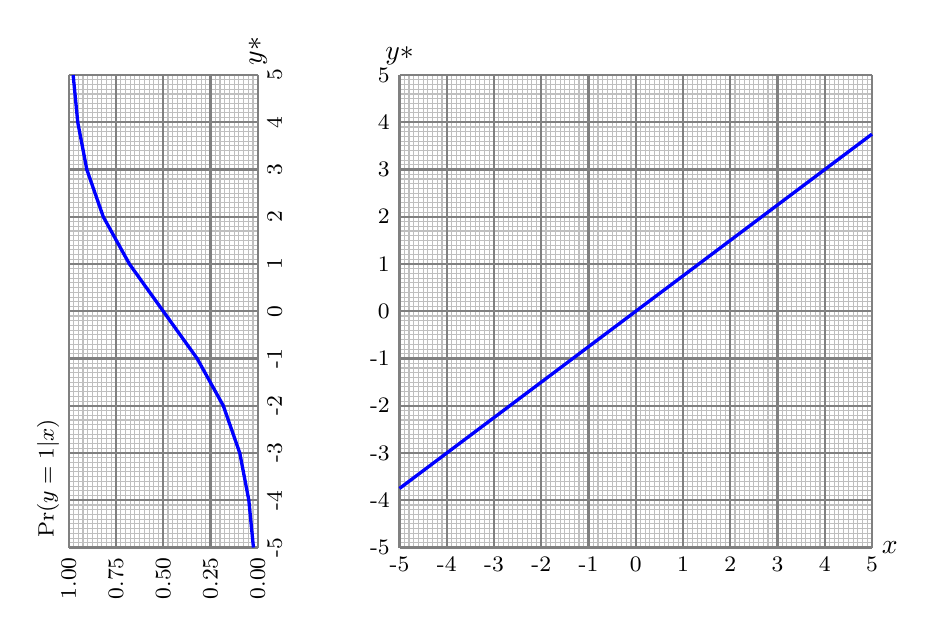
\begin{tikzpicture}[scale=0.6]
    
    % Pr(y)
    \draw [thin, step=0.1, lightgray] (-12,-5) grid (-8,5);
    \draw [thick, gray] (-12,-5) grid (-8,5);
    \node[left,rotate=90] () at (-8,-5) {\footnotesize 0.00};
    \node[left,rotate=90] () at (-9,-5) {\footnotesize 0.25};
    \node[left,rotate=90] () at (-10,-5) {\footnotesize 0.50};
    \node[left,rotate=90] () at (-11,-5) {\footnotesize 0.75};
    \node[left,rotate=90] () at (-12,-5) {\footnotesize 1.00};
    \foreach \y in {-5,...,5} {
        \node[below,rotate=90] () at (-8,\y) {\footnotesize \y};
    }
    \node[right,rotate=90] () at (-8,5) {$y\ast$};
    \node[above right,rotate=90] () at (-12,-5) {\footnotesize $\Pr(y=1|x)$};
    % paste0("(", -(8 + 4*round(plogis(0.75*(-5:5)),4)), ",", -5:5, ")", collapse = " -- ")
    \draw [very thick, blue] (-8.092,-5) -- (-8.1896,-4) -- (-8.3812,-3) -- (-8.7296,-2) -- (-9.2832,-1) -- (-10,0) -- (-10.7168,1) -- (-11.2704,2) -- (-11.6188,3) -- (-11.8104,4) -- (-11.908,5);
        
    % y*
    \draw [thin, step=0.1, lightgray] (-5,-5) grid (5,5);
    \draw [thick, gray] (-5,-5) grid (5,5);
    \node[right] () at (5,-5) {$x$};
    \node[above] () at (-5,5) {$y\ast$};
    \foreach \x in {-5,...,5} {
        \node[below] () at (\x,-5) {\footnotesize \x};
    }
    \foreach \y in {-5,...,5} {
        \node[left] () at (-5,\y) {\footnotesize \y};
    }
    % paste0("(", -5:5, ",", round(0.75*(-5:5),4), ")", collapse = " -- ")
    \draw [very thick, blue] (-5,-3.75) -- (-4,-3) -- (-3,-2.25) -- (-2,-1.5) -- (-1,-0.75) -- (0,0) -- (1,0.75) -- (2,1.5) -- (3,2.25) -- (4,3) -- (5,3.75);
    %\node[right,blue] () at (5,3.75) {$0 + 0.75x$};
    \end{tikzpicture}
    \end{center}
\end{frame}


\frame{
	\frametitle{Choosing a Link Function}
	\begin{itemize}\itemsep1em
	\item Based on expected distribution of the error term of $y\ast$
	\item Choice heavily influenced by convention rather than empirics
	\item Choice of link adds \textit{model dependence}!
		\begin{itemize}
		\item Expected influence of $x$ on $y$ now depends on choice of link
		\item Different link functions can yield different substantive and statistical results
		\item Generally, results are similar
		\end{itemize}
	\end{itemize}
}


\frame{
    \frametitle{Common Link Functions}
    \begin{center}
    {\renewcommand{\arraystretch}{1.75}
    \begin{tabular}{p{1in} p{1in} p{1in}}
    \textit{Name} & \textit{Link} & \textit{Inverse} \\ \hline
    Identity & $\mu$ & $y\ast$ \\
    Logit & $\ln\dfrac{\mu}{1-\mu}$ & $\dfrac{1}{1+e^{-y\ast}}$ \\
    Probit & $\Phi^{-1}(\mu)$ & $\Phi(y\ast)$ \\
    \hline
    \end{tabular}
    }
    \end{center}
    
    \begin{itemize}
    \item These are common for categorical outcomes
    \item Other types of outcomes will use different link functions
    \end{itemize}
}


\frame{
    \frametitle{Beyond Binary Outcomes}
    \begin{itemize}\itemsep1em
    \item The generalized linear model works for all kinds of outcomes, not just continuous or binary
    \item Consider, for example, a multi-category, ordered outcome variable
    \item In an \textit{ordered logit} model, we imagine a latent variable $y\ast$ and multiple cutpoints between categories of $y$
    \end{itemize}
}


\frame{
    \frametitle{Maximum Likelihood Estimation}
    \begin{itemize}\itemsep1em
    \item The \textit{generalized linear model} is a way of describing complex regression models
    \item Unlike OLS, there is no closed-form mathematical solution to GLM
        \begin{itemize}
        \item Recall a linear model can be expressed as a GLM
        \end{itemize}
    \item GLMs involve the big additional assumption of a distribution for the error term
    \item Maximum likelihood estimation is a way of estimating the GLM that makes use of that error distribution
    \end{itemize}    
}

\frame{
    \frametitle{Maximum Likelihood Estimation}
    \begin{itemize}\itemsep1em
    \item Choose an error distribution (which is described by various parameters)
    \item Select parameters as starting values
    \item Give a \textit{probability} of seeing each observation in our sample data given that distribution
    \item Combine those probabilities (i.e., likelihoods)
        \begin{itemize}
        \item Multiply the likelihoods
        \item Add the log-likelihoods
        \end{itemize}
    \item Repeat and pick the best guess from all of those that we test
    \end{itemize}
}


% assumptions



\subsection{Interpreting GLMs}
\frame{\tableofcontents[currentsection]}

\frame{
    \frametitle{Coefficients}
    \begin{itemize}\itemsep1em
    \item Coefficients express effect of $x$ on $y\ast$
    \item In logistic regression, this is a statement about the odds-ratio:
        $\hat{\beta} = \dfrac{\frac{p_1}{1-p_1}}{\frac{p_0}{1-p_0}}$
    \item Coefficients are hard to interpret \textit{substantively}
    \item Statistical significance is similar to OLS
    \end{itemize}
}

\frame{
    \frametitle{Predicted Outcomes}
	\begin{itemize}\itemsep1em
	\item In OLS, fitted values from the estimated regression equation are values of $y$
	\item In GLMs, fitted values are expressed for $y\ast$
	\item To interpret logit or probit, we transform to predicted probabilities
	\end{itemize}
}

\frame{
    \frametitle{Predicted Outcomes}
	\begin{itemize}\itemsep1em
	\item Definition: According to our coefficient estimates, what is $\Pr(\hat{y} = 1|X)$?
	\item To calculate this, we:
    	\begin{enumerate}
    	\item Calculate a fitted value on the latent/linear scale
    	\item Plug that fitted value into the inverse link function
    	\end{enumerate}
    \item In Stata, use \texttt{margins} and \texttt{predict}
        \begin{itemize}
        \item Probabilities are the default
        \item Use the \texttt{, xb} option for linear predictions
        \end{itemize}
    \end{itemize}
}


\frame{
    \frametitle{Marginal Effects}
    \begin{itemize}\itemsep1em
    \item A marginal effect refers to one of two quantities:
        \begin{itemize}
        \item For continuous variables: the partial derivative of the regression equation with respect to a specific variable
        \item For categorical variables: the difference $\Pr(y=1|x=1) - \Pr(y=1|x=0)$
        \end{itemize}
    \item In an OLS (with no interactions or other complex terms), the marginal effect is the coefficient itself
    \item In GLMs, this is more complicated
    \end{itemize}
}


\frame{
    \frametitle{Review: Partial Derivatives}
    \begin{itemize}\itemsep1em
    \item The partial derivative is the \textit{instantaneous} slope (or \textit{tangent}) of a line
    \item With one $x$ variable, this is just the slope of the line
    \item With > 1 $x$ variable, this is the conditional slope of the regression surface
        \begin{itemize}
        \item We hold other variables at some value see a ``slice'' of the regression surface
        \item The marginal effect is the slope of the slice
        \end{itemize}
    \end{itemize}
}


\frame{
	\frametitle{Simple regression surface}
	\begin{center}
	\begin{tikzpicture}
	    \draw[thick,->] (0,0,0) -- (6,0,0) node[anchor=north east]{$x$};
	    \draw[thick,->] (0,0,0) -- (0,4,0) node[anchor=north west]{$y$};
	    \draw[thick,->] (0,0,0) -- (0,0,5) node[anchor=south]{$z$};
	    \filldraw[draw=red,fill=red!20,opacity=0.5]
	        (0,2,0) -- (0,0,4) -- (5,-2,4) -- (5,0,0) -- cycle;
	    \draw<1> (3,3,0) node {$\hat{y} = \hat{\beta}_0 + \hat{\beta}_1 X + \hat{\beta}_2 Z$};
        \draw<2> (3,3,0) node {$\dfrac{\partial y}{\partial Z} = \hat{\beta}_2$};
	    \draw<2>[thick, red] (0,2,0) -- (0,0,4);
	    \draw<3> (3,3,0) node {$\dfrac{\partial y}{\partial X} = \hat{\beta}_1$};
	    \draw<3>[thick, blue] (0,2,0) -- (5,0,0);
	\end{tikzpicture}
	\end{center}
}



\frame{
    \frametitle{Discrete Changes}
    \begin{itemize}\itemsep1em
    \item Marginal effects are \textit{instantaneous changes}
    \item This makes sense for continuous variables
    \item For categorical (factor) variables, we often instead calculate a discrete change\\
        \begin{itemize}\itemsep1em
        \item $Pr(y=1|x=1) - Pr(y=1|x=0)$
        \item Marginal effect and discrete change are the same in OLS
        \end{itemize}
    \end{itemize}
}

\frame{
    \frametitle{Interaction Terms}
    \begin{itemize}\itemsep1em
    \item Due to the link function transformation, the marginal effect of $x$ depends on the value of $x$ and all other covariates
    \item This creates \textit{implicit} interactions
    \item We still have to include \textit{explicit} interaction terms to estimate heterogeneous effects (i.e., effect moderation)
    \end{itemize}
}


\frame{
	\frametitle{Logit vs. Probit}
	\begin{itemize}\itemsep1em
	\item<1-> Both constrain a continuous $y\ast$ to (0,1)
	\item<2-> Probabilities are symmetric
	\item<3-> Logit allows us to estimate odds-ratios
	\item<4-> Logit is maybe slightly more common in political science for what are probably just historical reasons
	\end{itemize}
}

\frame{
    \frametitle{Language of Interpretation}
    \begin{itemize}\itemsep1em
    \item How do we describe a marginal effect in OLS?
    \item<2-> In a binary outcome model, we use different language\\
    \item<3-> The substantive importance of an effect may depend on the level of $\Pr(y)$ at which it occurs\\
        \begin{itemize}\itemsep1em
        \item<4-> Small effect at $\Pr(y) = 0.01$ vs. $\Pr(y) = 0.48$
        \item<5-> Large positive effect when $\Pr(y)$ is always $> 0.6$
        \end{itemize}
    \item<6-> Substantive importance depends on variability and \textit{stickiness} of $x$
    \end{itemize}
}


\frame{
    \frametitle{Summarizing Marginal Effects}
    \begin{itemize}\itemsep1em
    \item We need to decide the values for all covariates that we will use in summarizing the marginal effect of our focal variable
    \item If our equation is: $y = g^{-1}(\beta_0 + \beta_1 x_1 + \beta_2 x_2 + \dots)$
    \item And we want to know the marginal effect of $x_1$, we need to hold $x_2$ at some specified value(s)
    \end{itemize}
}

\frame{
    \frametitle{3 Common Marginal Effect Summaries}
    \begin{enumerate}\itemsep2em
    \item Marginal Effects at the Mean (MEMs)
    \item Marginal Effects at Representative Values (MERs)
    \item Average Marginal Effects (AMEs)
    \end{enumerate}
}


\frame{
    \frametitle{MEM}
    \begin{itemize}\itemsep1em
    \item We are interested in the ME of $x_1$
    \item We hold all other covariates at their respective means
    \item For example, we interested in the ME of \textit{knowledge}, we hold \textit{education} at its mean
    \item<2-> Does this make sense for categorical values (e.g., gender)?
    \end{itemize}
}

\frame{
    \frametitle{MERs}
    \begin{itemize}\itemsep1em
    \item The means of the covariates may not be meaningful
    \item We hold those covariates at various interesting values
        \begin{itemize}
        \item ME of $x$ for a high-school educated female
        \item ME of $x$ for a university-educated male
        \item etc.
        \end{itemize}
    \item Helpful because we may also be interested in $\Pr(y=1)$ for these cases
    \end{itemize}
}

\frame{
    \frametitle{AMEs}
    \begin{itemize}\itemsep1em
    \item We may not only be interested in MEs at particular values
    \item We may want a summary measure of the effect of $x$ for our sample as a whole
    \item The \textit{average marginal effect} calculates the MER for every observation in our data, then averages those ME values
    \item This is Stata's default behavior when using:\\ \texttt{margins, dydx(*)}
    \end{itemize}
}


\frame{
    \frametitle{AMEs: An Example}
    \begin{itemize}
    \item Model effects of gender \& education on trust
    \item Calculate ME for each observation
    \item Average to obtain AME
    \end{itemize}
    
    \visible<2->{
    \begin{center}
    \begin{tabular}{lllrr}
    Obs. & Gender & Degree & $ME(Gender)$ & $ME(Degree)$ \\
    \hline 
    1 & 1 & 1 & 0.10 & 0.25 \\
    2 & 1 & 1 & 0.10 & 0.25 \\
    3 & 1 & 0 & 0.20 & 0.15 \\
    4 & 0 & 1 & 0.30 & -0.25 \\
    5 & 0 & 0 & 0.10 & -0.40 \\
    \hline 
    AME & -- & -- & \only<3->{0.16} & \only<4->{0.00} \\
    \hline 
    \end{tabular}
    \end{center}
    }
}

\frame{
    \frametitle{Statistical Uncertainty}
    \begin{itemize}\itemsep1em
    \item Always express statistical uncertainty for:
        \begin{itemize}
        \item Coefficients
        \item Predicted probabilities
        \item Marginal effects
        \end{itemize}
    \item Significance of coefficients and marginal effects may vary
    \item Marginal effects may only differ from 0 on a subset of the range of $x$
    \item Be cautious about extrapolation
    \end{itemize}
}


\frame{
    \frametitle{Aside: Discrete Effects}
    \begin{itemize}\itemsep1em
    \item Discrete effects can also be calculated for continuous variables
    \item Requires choosing a substantively meaningful change in $x$
    \item \textbf{Caution!} Not necessary equal:\\
        \begin{itemize}\itemsep1em 
        \item $\Pr(y = 1|x = 5) - \Pr(y = 1|x = 1)$
        \item ME at $x = 5$ (MER)
        \item ME at $x = 1$ (MER)
        \item ME at $x = 3$ (AME/MEM)
        \end{itemize}
    \end{itemize}
}

\begin{frame}[fragile]
    \frametitle{Discrete and Marginal Effects}
    \vspace{-1.5em}
    \begin{center}
    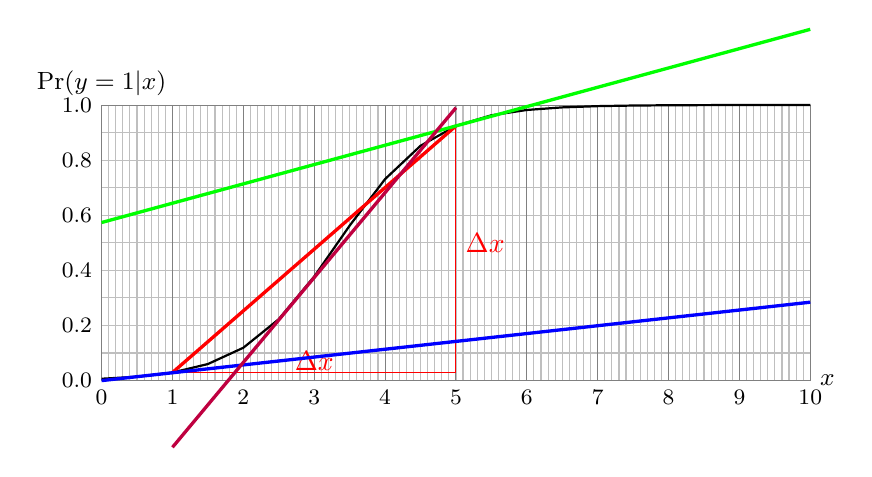
\begin{tikzpicture}[yscale=3.5, xscale=0.9]
    \draw [thin, step=0.1, lightgray] (0,0) grid (10,1);
    \draw [thin, gray] (0,0) grid (10,1);
    \node[right] () at (10,0) {\small $x$};
    \node[above] () at (0,1) {\small $\Pr(y=1|x)$};
    \foreach \x in {0,...,10} {
        \node[below] () at (\x,0) {\footnotesize \x};
    }
    \foreach \y in {0.0,0.2,0.4,0.6,0.8,1.0} {
    \node[left] () at (0,\y) {\footnotesize \y};
    }
    % paste0("(", seq(0,10,by=0.5), ",", round(plogis(-5 + 1.5*(seq(0,10,by=0.5))),4), ")", collapse = " -- ")
    \draw [thick, black] (0,0.0067) -- (0.5,0.0141) -- (1,0.0293) -- (1.5,0.0601) -- (2,0.1192) -- (2.5,0.2227) -- (3,0.3775) -- (3.5,0.5622) -- (4,0.7311) -- (4.5,0.852) -- (5,0.9241) -- (5.5,0.9627) -- (6,0.982) -- (6.5,0.9914) -- (7,0.9959) -- (7.5,0.9981) -- (8,0.9991) -- (8.5,0.9996) -- (9,0.9998) -- (9.5,0.9999) -- (10,1);
    
    % discrete change
    % plogis(-5 + (1.5 * 1))
    % plogis(-5 + (1.5 * 5))
    \draw<2> [red] (1,0.0293) -- (5,0.0293);
    \draw<2> [red] (5,0.0293) -- (5,0.9241);
    \draw<2> [very thick, red] (1,0.0293) -- (5,0.9241);
    \node<2>[right,red] () at (5, 0.5) {$\Delta x$};
    \node<2>[above,red] () at (3, 0) {$\Delta x$};
    
    % ME at x = 1
    % dlogis(-5 + (1.5 * 1))
    \draw<3> [very thick, blue] (0,0) -- (10,0.2845);
    
    % ME at x = 5
    % dlogis(-5 + (1.5 * 5))
    \draw<4> [very thick, green] (0,0.5736) -- (10,1.2746);
    
    % ME at x = 3
    % dlogis(-5 + (1.5 * 3))
    \draw<5> [very thick, purple] (1,-0.242) -- (5,0.99);
        
    
    \end{tikzpicture}
    \end{center}
    
    \vspace{-2em}
    
    {\small
    \begin{itemize}
    \item<2-6> Discrete change: 0.9241 - 0.0293 = 0.8948
    \item<3-6> ME at $x = 1$: 0.0285
    \item<4-6> ME at $x = 5$: 0.0701
    \item<5-6> ME at $x = 3$: 0.2350
    \end{itemize}
    }
    
\end{frame}

\frame{
    \frametitle{Language of Interpretation}
    \begin{itemize}\itemsep0.5em
    \item \textbf{Discrete effect}: A change in $x$ from $a$ to $b$ results in an increase in the predicted probability that $y$ equals 1 of 0.89, which is a substantively large and statistically significant effect.
    \item \textbf{Marginal effect}: The marginal effect of $x$ on the probability that $y$ = 1 when $x$ equals $a$ is 0.07, which is a large and statistically significant effect. The predicted probability of $y$ at this point is only 0.03, however, suggesting $x$ may be substantively unimportant for cases with this value of $x$.
    \end{itemize}
}


\frame{
    \frametitle{Summary}
    \begin{itemize}\itemsep1em
    \item Many ways to summarize GLMs
        \begin{itemize}
        \item Coefficients
        \item Predicted probabilities
        \item Marginal effects
        \item Discrete effects
        \end{itemize}
    \item<2-> Graphs help interpretation considerably
    \item<3-> There's no single correct way of summarizing a complex model
    \end{itemize}
}




\section{Panel Studies and Regression}
\frame{\tableofcontents[currentsection]}

\frame{\frametitle{}}

% panel surveys in concept
% contrast with repeated cross-sections

% talk about panel regression
% multi-level modeling






\frame{
    \frametitle{Pooled Estimator}
    \begin{itemize}\itemsep1em
    \item $y_{it} = \beta_0 + \beta_1 x_{it} + \dots + \epsilon_{it}$
    \item Ignores panel structure (interdependence)
    \item Ignores heterogeneity between units
    \item But, we can actually easily estimate and interpret this model!
    \item Estimation uses ``generalized estimating equations'' (GEE)
    \item Note: Also called \textit{population-averaged} model
    \end{itemize}
}

\frame{
    \frametitle{Pooled Estimator}
    \begin{itemize}\itemsep1em
    \item Continuous outcomes:\\
        $y_{it} = \beta_0 + \beta_1 x_{it} + \dots + \epsilon_{it}$
    \item Binary outcomes:\\
        $y_{it}\ast = \beta_0 + \beta_1 x_{it} + \dots + \epsilon_{it}$\\
        $y_{it} = 1$ if $y_{it}\ast > 0$, and 0 otherwise
    \item Link functions are the same in panel as in cross-sectional
        \begin{itemize}
        \item Logit
        \item Probit
        \end{itemize}
    \item Use clustered standard errors
    \end{itemize}
}





\frame{
    \frametitle{Respecting the Panel Structure}
    \begin{itemize}\itemsep1em
    \item With a panel structure, $\epsilon_{it}$ can be decomposed into two parts:
        \begin{itemize}
        \item $\upsilon_{it}$
        \item $u_i$
        \end{itemize}
    \item If we assume $u_i$ is unrelated to $X$: fixed effects
    \item If we allow a correlation: random effects
    \end{itemize}
}

\frame{
    \frametitle{Fixed Effects Estimator}
    \begin{itemize}\itemsep1em
    \item This gives us:\\
        \begin{equation}
        \begin{array}{ll}
        y_{it} & = \beta_{0} + \beta_1 x_{it} + \dots + \upsilon_{it} + u_i\\
        y_{it} & = \beta_{0i}d_{it} + \beta_1 x_{it} + \dots + \upsilon_{it}
        \end{array}
        \end{equation}
    \item Varying intercepts (one for each unit)
    \item Can generalize to other specifications (e.g., fixed period effects)
    \end{itemize}
}


\frame{
    \frametitle{Fixed Effects Estimator}
    \begin{itemize}\itemsep1em
    \item Fixed effects terms absorb all time-invariant between-unit heterogeneity
    \item Effects of time-invariant variables cannot be estimated
    \item Each unit is its own control (``within'' estimation)
    \item Two ways to estimate this:
        \begin{itemize}
        \item Unconditional maximum likelihood
        \item Conditional maximum likelihood
        \end{itemize}
    \item Both are problematic
    \end{itemize}
}

\frame{
    \frametitle{Fixed Effects Estimator}
    \begin{itemize}\itemsep1em
    \item Unconditional maximum likelihood
        \begin{itemize}
        \item From OLS: dummy variables for each unit
        \item Number of parameters to estimate increases with sample size
        \item For logit/probit: \textit{incidental parameters problem}
        \item Estimate become inconsistent
        \end{itemize}
    \item Conditional maximum likelihood
        \begin{itemize}
        \item From OLS: ``De-meaned'' data to avoid estimating unit-specific intercepts
        \item For logit: condition on $Pr(Y_i=1)$ across all $t$ periods
        \item Does not work for probit!
        \end{itemize}
    \end{itemize}
}

\frame{
    \frametitle{Conditional MLE}
    \begin{itemize}\itemsep1em
    \item Estimates only based on units that change in $Y$
    \item Effects of time-invariant variables are not estimable
    \item Observations with time-invariant outcome are dropped
    \item<2-> Estimation of two-wave panel using fixed-effects logistic regression is same as a pooled logistic regression where the outcome is direction of change regressed on time-differenced explanatory variables
    \end{itemize}
}

\frame{
    \frametitle{Fixed Effects Estimator}
    \begin{itemize}\itemsep1em
    \item Interpretation is difficult
    \item Use \texttt{predict} to get fitted values on the latent scale
    \item \texttt{margins, dydx()} is also problematic
        \begin{itemize}
        \item Use \texttt{, predict(xb)} to obtain log-odds marginal effects
        \item Use \texttt{, predict(pu0)} to assume fixed effect is zero
        \item Neither of those is the default
        \end{itemize}
    \end{itemize}
}



\frame{
    \frametitle{Random Effects Estimator}
    \begin{itemize}\itemsep1em
    \item If we are willing to assume that unit-specific error term is uncorrelated with other variables
    \item Why might this not be the case?
    \item<2-> Pooled estimator also makes this assumption
    \item<2-> But that estimator ignores panel structure (non-independence)
    \end{itemize}
}

\frame{
    \frametitle{Estimation hell!}
    \begin{itemize}\itemsep0.5em
    \item<2-> Due to \textit{incidental parameters problem} we cannot consistently estimate both the regression coefficients and the unit-specific effects
    \item<3-> We have to make some assumptions about the unit-specific error terms
    \item<3-> But assumptions get us to a likelihood function that can only be maximized via \textit{integration} of a complicated function
    \item<3-> Quadrature (a form of numerical approximation of an integral) is therefore used (costly!)
    \end{itemize}
}

\frame{
    \frametitle{Random Effects Estimator}
    \begin{itemize}\itemsep1em
    \item Can be used with logit or probit
    \item Interpretation is messy because unit-specific error terms are unobserved
    \item Thus marginal effects calculation must make an assumption of about the random effects:
        \begin{itemize}
        \item Predict log-odds: \texttt{margins, dydx(*)}
        \item Assume they are 0: \texttt{, predict(pu0)}
        \end{itemize}
    \end{itemize}
}


\frame{
    \frametitle{Random versus Fixed Effects}
    \begin{itemize}\itemsep1em
    \item Different assumptions
    \item Very different estimation strategies
        \begin{itemize}
        \item These are consequential for interpretation
        \end{itemize}
	\item Common practice is to estimate multiple specifications
    \end{itemize}
}


\frame{
    \frametitle{Reminder!}
    \begin{itemize}\itemsep1em
    \item Some outcomes are binary but are constant before and after an ``event''
        \begin{itemize}
        \item Individual graduates from university
        \item Country transitions to democracy
        \end{itemize}
    \item We can analyze these using binary outcome panel models \textit{or} using event-history methods from last week
    \item Either might be appropriate, depending on the research question, hypothesis, and data
    \end{itemize}
}



\frame{
    \frametitle{Ordered Outcome Models}
    \begin{itemize}\itemsep1em
    \item Estimators exist, but only random effects is implemented in Stata
        \begin{itemize}
        \item Logit and probit available
        \end{itemize}
    \item Other possible analysis strategies:
        \begin{itemize}\itemsep0.5em
        \item Use a linear panel specification
        \item Estimate a pooled model with clustered SEs
        \item Recode categories to binary and use
        \item Use a mixed effects specification
        \end{itemize}
    \end{itemize}
}


\frame{
    \frametitle{Standard Errors}
    \begin{itemize}\itemsep1em
    \item Standard errors can be complicated
    \item For pooled model, use standard errors clustered by unit
        \begin{itemize}
        \item \texttt{vce(robust)}
        \item \texttt{vce(cluster id)}
        \end{itemize}
    \item For random effects, you may want bootstrapped standard errors
    \item Always check for robustness
    \end{itemize}
}

\frame{
    \frametitle{Interpretation: Quick Review}
    \begin{itemize}\itemsep1em
    \item Usual rules don't apply
    \item Estimation via an MLE variant usually means marginal effects are undefined
    \item Depending on model specification, predicted values may also be \textit{conditional}
    \item We have to make further assumptions to create an interpretable quantity of interest from the model
    \end{itemize}
}

\frame{
    \frametitle{Intepretation: Trade-offs}
    \begin{itemize}\itemsep1em
    \item Analytic trade-off between model choice and interpretability
    \item Pooled estimates are interpretable in conventional ways, but use assumptions
        \begin{itemize}
        \item Ignores panel structure
        \item No unobserved confounding/heterogeneity
        \end{itemize}
    \item Other models are harder to estimate and interpret, but may be more ``correct,'' though:
        \begin{itemize}
        \item RE assumes heterogeneity is not confounding
        \item FE disallows effects of time-invariant variables
        \end{itemize}
    \end{itemize}
}

\frame{
    \frametitle{Mixed Effects/\\Hierarchical Models}
    \begin{itemize}\itemsep1em
    \item We can also estimate mixed effects models for non-linear outcomes
    \item This can be easier analytically than other panel model specifications
    \item These models also make sense when you have data that have a true hierarchical structure (such as persons within times within countries)
	\end{itemize}

}


\frame{}

\frame{\tableofcontents}



\appendix
\frame{}

\end{document}
